\subsection{Hamming}
\textbf{Experimento 1}. Es importante señalar que la asignación de valores se realizo a través de un archivo de texto llamado \emph{entrada\_hamming.txt}
\begin{figure}[H]
    \begin{center}
        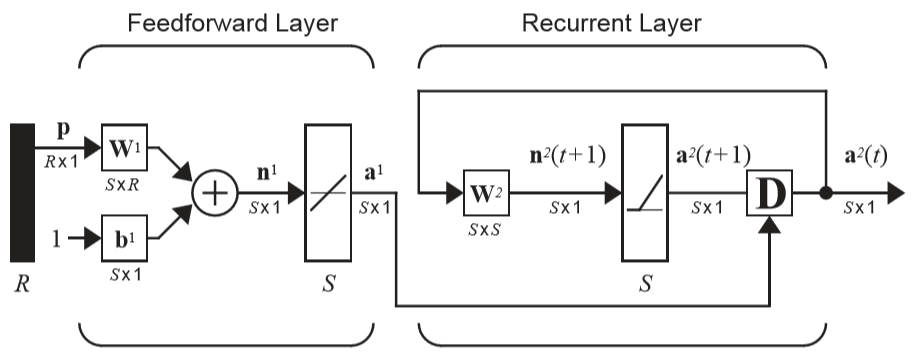
\includegraphics[width=16cm]{img/hamming/diagrama.png}
        \caption{Estructura de la red de Hamming. \cite{libro1}}
        \label{fig:hamming-diagrama2}
    \end{center}
\end{figure}
Para hacer la primera prueba sobre la red Hamming se utilizo el siguiente conjunto de vectores prototipo.
\[ \left\lbrace \boldsymbol{p_1} = \left[\begin{array}{c}-1\\ 1\\ -1\end{array}\right], \boldsymbol{p_2} = \left[\begin{array}{c}-1\\ -1\\ 1\end{array}\right], \boldsymbol{p_3} = \left[\begin{array}{c}1\\ 1\\ -1\end{array}\right], \boldsymbol{p_4} = \left[\begin{array}{c}1\\ -1\\ -1\end{array}\right] \right\rbrace \]
Y el vector de a clasificar fue el siguiente.
\[ \boldsymbol{p} = \left[\begin{array}{c}-1\\ 1\\ -1\end{array}\right] \]
Por lo que la arquitectura definida en la figura \ref{fig:hamming-diagrama2} tiene los siguientes valores.
\begin{align*}
R = 3 \implies \boldsymbol{b^1} = \left[\begin{array}{c}3\\ 3\\ 3\end{array}\right] && S = 4 && \boldsymbol{W^1} = \left[\begin{array}{c}\boldsymbol{p^{T}_1}\\ \boldsymbol{p^{T}_2}\\ \boldsymbol{p^{T}_3} \\ \boldsymbol{p^{T}_4}\end{array}\right]
\end{align*}
Al aplicar estos valores a nuestra red la capa recurrente termino en la iteración 13 y convergió exitosamente a la clase 1 que es la que se esperaba que convergiera.
%modelo matemático, arquitectura, conjunto de entrenamiento, condición de finalización, valores finales de w y bias
\begin{figure}[H]
    \begin{center}
        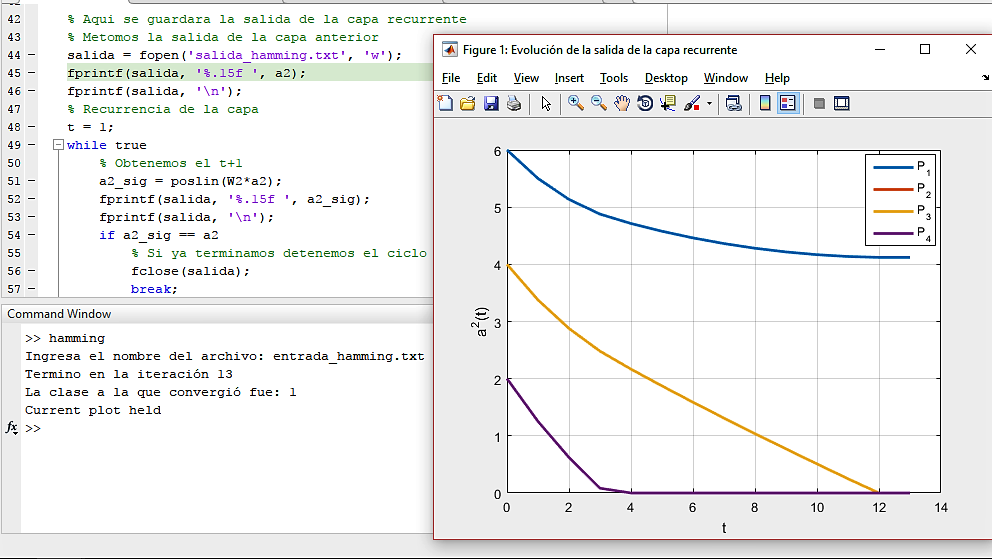
\includegraphics[width=16cm]{img/hamming/hamming1.png}
        \caption{Prueba 1 de la red Hamming.}
        \label{fig:hamming1}
    \end{center}
\end{figure}
En la figura \ref{fig:hamming1} se puede observar que solo la curva asociada a la neurona 1 de la capa recurrente que corresponde al vector prototipo 1 es la única que tiene un valor distinto de 0.
\newline
\textbf{Experimento 2.}
En esta segunda prueba se utilizo el siguiente conjunto de vectores prototipo.
\[ \left\lbrace \boldsymbol{p_1} = \left[\begin{array}{c}1\\ -1\\ -1 \\ -1 \end{array}\right], \boldsymbol{p_2} = \left[\begin{array}{c}-1\\ -1\\ -1 \\ 1 \end{array}\right] \right\rbrace \]
El vector de prueba a clasificar fue el siguiente.
\[ \boldsymbol{p} = \left[\begin{array}{c}1\\ 1\\ -1 \\ -1\end{array}\right] \]
Los valores fueron ingresados mediante un archivo de texto llamado \emph{entrada\_hamming2.txt}. Esto dio como resultado que los valores de la red Hamming de la figura \ref{fig:hamming-diagrama2} sean los siguientes.
\begin{align*}
R = 4 \implies \boldsymbol{b} = \left[\begin{array}{c}4 \\4\end{array}\right] && S = 2 && \boldsymbol{W} = \left[\begin{array}{c}\boldsymbol{p^{T}_1}\\ \boldsymbol{p^{T}_2}\end{array}\right]
\end{align*}
\begin{figure}[H]
    \begin{center}
        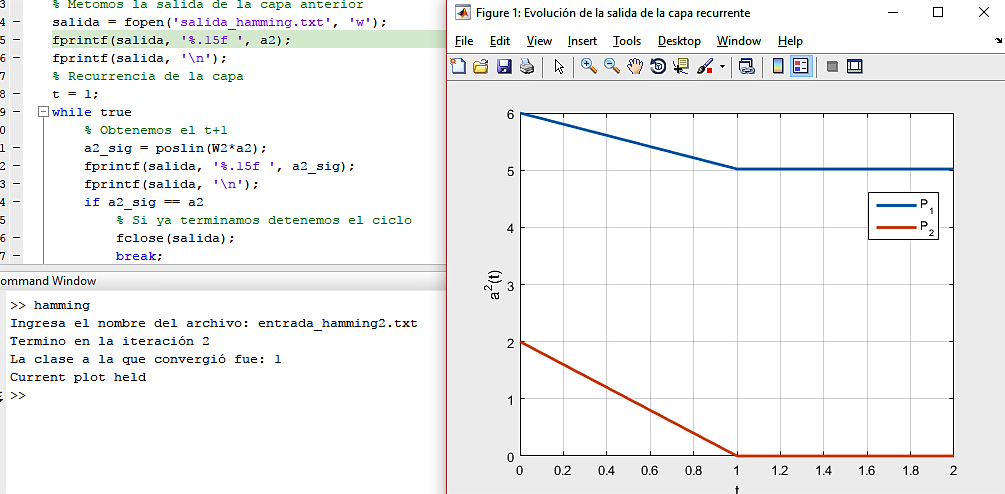
\includegraphics[width=16cm]{img/hamming/hamming2.png}
        \caption{Prueba 2 de la red Hamming.}
        \label{fig:hamming2}
    \end{center}
\end{figure}
Después del procesamiento de estos datos se pudo clasificar correctamente el vector de entrada, a la red le tomo dos iteraciones logar converger y a la clase a la que convergió fue la 1, esto se puede observar a detalle en la evolución de las salidas de la capa recurrente que se encuentra en la figura \ref{fig:hamming2}.
\newline
\textbf{Experimento 3.} En este ultimo experimento se utilizo un archivo llamado \emph{entrada\_hamming3.txt} para poder ingresar los datos a la red. El conjunto de vectores prototipo fue el siguiente.
\[ \left\lbrace \boldsymbol{p_1} = \left[\begin{array}{c}-1\\ 1\\ 1 \\ 1 \\ 1 \end{array}\right], \boldsymbol{p_2} = \left[\begin{array}{c}-1\\ -1\\ 1 \\ -1 \\ 1 \end{array}\right], \boldsymbol{p_3} = \left[\begin{array}{c}1\\ 1\\ -1 \\ -1 \\ -1 \end{array}\right], \boldsymbol{p_4} = \left[\begin{array}{c}-1\\ -1\\ -1 \\ -1 \\ -1 \end{array}\right], \boldsymbol{p_5} = \left[\begin{array}{c}1\\ 1\\ 1 \\ 1 \\ 1 \end{array}\right] \right\rbrace \]
El vector de prueba que se utilizo fue.
\[ \boldsymbol{p} = \left[\begin{array}{c}1\\ -1\\ 1 \\ -1 \\ 1\end{array}\right] \]
El utilizar estos valores produjo que la arquitectura de la figura \ref{fig:hamming-diagrama2} tuviera los siguientes valores.
\begin{align*}
R = 5 \implies \boldsymbol{b} = \left[\begin{array}{c}5 \\5 \\ 5 \\ 5 \\ 5\end{array}\right] && S = 5 && \boldsymbol{W} = \left[\begin{array}{c}\boldsymbol{p^{T}_1}\\ \boldsymbol{p^{T}_2} \\ \boldsymbol{p^{T}_3} \\ \boldsymbol{p^{T}_4} \\ \boldsymbol{p^{T}_5}\end{array}\right]
\end{align*}
\begin{figure}[H]
    \begin{center}
        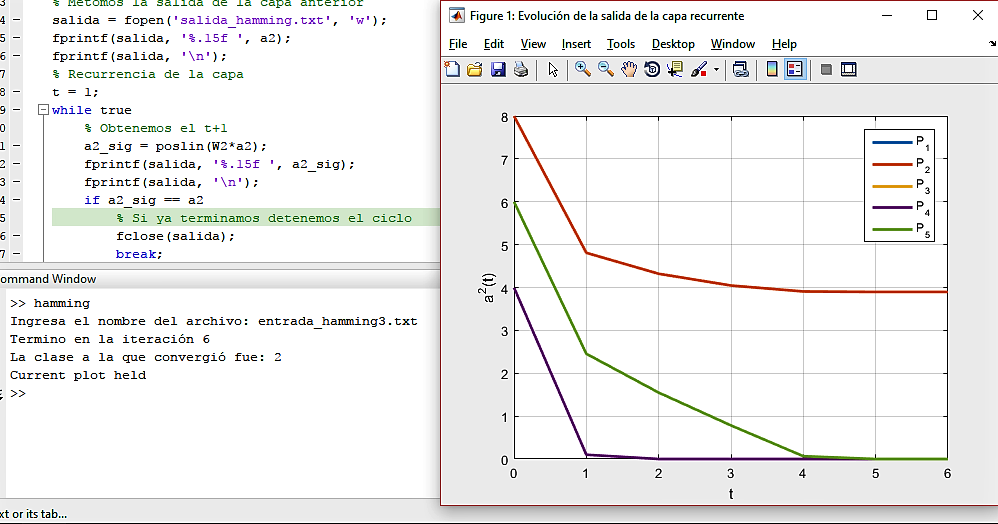
\includegraphics[width=16cm]{img/hamming/hamming3.png}
        \caption{Prueba 3 de la red Hamming.}
        \label{fig:hamming3}
    \end{center}
\end{figure}
Como se puede observar en la figura \ref{fig:hamming3} la red pudo converger a un resultado satisfactorio en la iteración 6 dando como resultado que el vector de prueba perteneciera a la clase 2 debido a que es la única salida que tiene un valor diferente a 0.
\newpage